\documentclass[12pt]{article}
\usepackage{amsmath}
\usepackage{graphicx}
\usepackage{array}

\graphicspath{ {./images/} }

\title{Argent Smart Wallet Specification}
\author{v2.5}
\date{\today}


\begin{document}

\maketitle
%\tableofcontents{}

%%%%%%%%%%%%%%%%%%%%%%%%%%%%%%%%%%%%%%%%%%%%%%%%%%%%%%%%%%%%%%%%%%%%%%%%%%%%%%%%%%%%%%%%%%%%%%%%%%%
%%%%%%%%%%%%%%%%%%%%%%%%%%%%%%%%%%%%%%%%%%%%%%%%%%%%%%%%%%%%%%%%%%%%%%%%%%%%%%%%%%%%%%%%%%%%%%%%%%%
\section{Specifications}

%%%%%%%%%%%%%%%%%%%%%%%%%%%%%%%%%%%%%%%%%%%%%%%%%%%%%%%%%%%%%%%%%%%%%%%%%%%%%%%%%%%%%%%%%%%%%%%%%%%
\subsection{Introduction}

The Argent wallet is an Ethereum Smart Contract based mobile wallet. The wallet's user keeps an Ethereum account (Externally Owned Account) secretly on his mobile device. This account is set as the owner of the Smart Contract. User's assets (e.g. ETH, ERC20, ERC721 or ERC1155 tokens) are stored on the Smart Contract. With that model, logic can be added to the wallet to improve both the user experience and the wallet security. For instance, the wallet is guarded, recoverable, transferable, lockable and upgradable.

%%%%%%%%%%%%%%%%%%%%%%%%%%%%%%%%%%%%%%%%%%%%%%%%%%%%%%%%%%%%%%%%%%%%%%%%%%%%%%%%%%%%%%%%%%%%%%%%%%%
\subsection{Guardians}

The wallet security model is based on the ability to add \textit{guardians}. A guardian is an account (EOA or smart contract) that has been given permission by the wallet's owner to execute certain specific operations on their wallet. In particular guardians can lock, unlock, and trigger a recovery procedure on the wallet as well as approve the execution of transactions to unknown accounts or the creation of a session key.

We do not impose restrictions on who or what guardians are. They can be a friend's Argent wallet, a friend's EOA, a hardware wallet, or even a paid third-party service.

Adding a guardian is an action triggered by the wallet owner. While the first guardian is added immediately when the wallet is created, all subsequent additions must be confirmed after 36 hours and no later than 48 hours after the addition was requested. This confirmation window ensures that a pending addition will be canceled (expire) should the wallet be locked or recovered.

Removing a guardian is an action triggered by the wallet owner. It must always be confirmed after 36 hours and no later than 48 hours after the removal was requested. This leaves the legitimate wallet owner enough time to notice and prevent the appointment of an illegitimate guardian (or the dismissal of a legitimate guardian) in case the owner lost control over their mobile device.

%%%%%%%%%%%%%%%%%%%%%%%%%%%%%%%%%%%%%%%%%%%%%%%%%%%%%%%%%%%%%%%%%%%%%%%%%%%%%%%%%%%%%%%%%%%%%%%%%%%
\subsection{Locking}

In case the wallet owner suspects his account (i.e. device) is compromised (lost, stolen, ...), he can ask any of his guardians to lock the wallet for a security period of 5 days. Once the wallet is locked only a limited set of actions can be operated on the wallet, namely the recovery procedure, the unlock procedure, or the revocation of Guardians. All other operations (add guardian, assets transfer, ...) are blocked.

To unlock a wallet before the end of the security period, any guardian should trigger a wallet unlock.

%%%%%%%%%%%%%%%%%%%%%%%%%%%%%%%%%%%%%%%%%%%%%%%%%%%%%%%%%%%%%%%%%%%%%%%%%%%%%%%%%%%%%%%%%%%%%%%%%%%
\subsection{Recovery}

Wallet recovery is a process requested by a user who asserts ownership of a wallet while not being in possession of the owner key. A successful recovery sets a new account as the wallet owner. This process should be validated by the wallet's guardians to be executed and thus requires the wallet to have at least 1 guardian. Once a recovery has been executed it may be finalised after 48 hours, unless it has been cancelled.

The number of signatures needed to execute a recovery is given by
\begin{equation*}
    \left\lceil {\frac{n}{2}} \right\rceil
\end{equation*}
where $n$ is the total number of guardians and $\lceil\rceil$ is the ceiling function.

A recovery can be cancelled before finalisation. The number of signatures (owner and/or guardians) needed to cancel a recovery is given by
\begin{equation*}
    \left\lceil {\frac{n+1}{2}} \right\rceil
\end{equation*}
where $n$ is the total number of guardians when the recovery was executed.

Once a recovery is started the wallet is automatically locked. The wallet can only be unlock by finalising or cancelling the ongoing procedure, i.e. guardians cannot unlock during a recovery.

%%%%%%%%%%%%%%%%%%%%%%%%%%%%%%%%%%%%%%%%%%%%%%%%%%%%%%%%%%%%%%%%%%%%%%%%%%%%%%%%%%%%%%%%%%%%%%%%%%%
\subsection{Ownership Transfer}

In addition to recovery it is possible for a user to transfer ownership of his wallet to a new device while still being in possession of the actual phone. This transfer is immediate to avoid service interruption but must be approved by guardians. The number of required signatures is given by
\begin{equation*}
    1+\left\lceil {\frac{n}{2}} \right\rceil
\end{equation*}
where the first signature is the owner and $n$ is the total number of guardians.

%%%%%%%%%%%%%%%%%%%%%%%%%%%%%%%%%%%%%%%%%%%%%%%%%%%%%%%%%%%%%%%%%%%%%%%%%%%%%%%%%%%%%%%%%%%%%%%%%%%
\subsection{Multi-Call}

The wallet can interact with the ethereum eco-system to e.g. send an asset or interact with the smart-contracts of a decentralized application through multi-calls. A multi-call is a sequence of transactions executed by the wallet one after the other and such that the multi-call fails if any of the transaction fails.

By design the wallet will block a multi-call unless one of the following conditions is satisfied:
\begin{enumerate}
    \item the multicall is triggered by the wallet owner and each transaction of the multi-call:
    \begin{itemize}
        \item transfers or approves an asset (ETH, ERC20, ERC721, ERC1155) to a trusted contact see Section \ref{sec:trusted-contacts}
        \item transfers or approves an asset (ETH, ERC20, ERC721, ERC1155) or calls an authorised Dapp see Section \ref{sec:authorised-dapps}
    \end{itemize}
    \item the multicall is approved by the owner and a majority of guardians see Section \ref{sec:guardian-approval} 
    \item the multicall is executed with a valid session key see Section \ref{sec:session}
\end{enumerate}

%%%%%%%%%%%%%%%%%%%%%%%%%%%%%%%%%%%%%%%%%%%%%%%%%%%%%%%%%%%%%%%%%%%%%%%%%%%%%%%%%%%%%%%%%%%%%%%%%%%
\subsection{Trusted Contacts}
\label{sec:trusted-contacts}

The wallet keeps a list of trusted addresses managed by the wallet owner.
Adding an address to this list is an action triggered by the wallet owner and takes 36 hours to be effective. Removing an address is triggered by the owner and is immediate.

Interracting with a trusted contact to e.g. send an asset, can be triggered by the wallet owner and does not require any additional authorisation. 

%%%%%%%%%%%%%%%%%%%%%%%%%%%%%%%%%%%%%%%%%%%%%%%%%%%%%%%%%%%%%%%%%%%%%%%%%%%%%%%%%%%%%%%%%%%%%%%%%%%
\subsection{Dapp Registry}
\label{sec:authorised-dapps}

In addition to trusted contacts, the wallet supports 2 registries of addresses that have been authorised by Argent.

The first registry is enabled by default (opt-out) for all wallets and contains all the dapps that are natively integrated in the Argent client application (Paraswap, Compound, Maker, Aave, etc). The second registry is disabled by default (opt-in) and contains a list of curated dapps that the user can access through WalletConnect.

Each registry entry is a mapping between an authorised address and a filter containing the set of conditions that a transaction from a wallet to the authorised address must satisfy.
Adding or removing an entry in a registry is a timelocked operations that can only be initiated by the Argent multisig.
The timelock is set to 7 days to give enough time for a user to disable the correspoding registry should they not approve the new addition. 

Enabling a registry for a wallet requires guardian approvals and the number of required signatures is given by
\begin{equation*}
    1+\left\lceil {\frac{n}{2}} \right\rceil
\end{equation*}
where the first signature is the owner and $n$ is the total number of guardians. Disabling a registry can be executed by the wallet owner alone.

Interacting with an authorised dapp to e.g. invest an asset in a DeFi protocol, can be triggered by the owner provided that the corresponding registry is enabled for the wallet and the transaction passes the associated filter.

%%%%%%%%%%%%%%%%%%%%%%%%%%%%%%%%%%%%%%%%%%%%%%%%%%%%%%%%%%%%%%%%%%%%%%%%%%%%%%%%%%%%%%%%%%%%%%%%%%%
\subsection{Guardian Approval}
\label{sec:guardian-approval}

Any sequence of transactions (multi-call) can be executed by the wallet owner provided that they obtain approval from their guardians. The number of required signatures is given by
\begin{equation*}
    1+\left\lceil {\frac{n}{2}} \right\rceil
\end{equation*}
where the first signature is the owner and $n$ is the total number of guardians.

%%%%%%%%%%%%%%%%%%%%%%%%%%%%%%%%%%%%%%%%%%%%%%%%%%%%%%%%%%%%%%%%%%%%%%%%%%%%%%%%%%%%%%%%%%%%%%%%%%%
\subsection{Session}
\label{sec:session}

Users that plan to execute many transactions in a given time window while only requiring their guardian approval once can do so by creating a session. A session defines a temporary session key that can be used to execute any multi-call for as long as the session key is valid. The duration of the session is defined by the owner when the session is created and the session key will automatically become invalid at the end the session.

The number of required signatures to start a session is given by
\begin{equation*}
    1+\left\lceil {\frac{n}{2}} \right\rceil
\end{equation*}
where the first signature is the owner and $n$ is the total number of guardians.

The wallet owner can always close a session before it's expiration.

%%%%%%%%%%%%%%%%%%%%%%%%%%%%%%%%%%%%%%%%%%%%%%%%%%%%%%%%%%%%%%%%%%%%%%%%%%%%%%%%%%%%%%%%%%%%%%%%%%%
\subsection{Upgradability}

The wallet is upgradable to add new features and fix potential bugs. The choice of whether to upgrade or not a wallet is left to the wallet owner. In particular, it is not possible for a centralised party such as Argent to force a wallet upgrade and change an implementation that is assumed to be immutable by the owner.

%%%%%%%%%%%%%%%%%%%%%%%%%%%%%%%%%%%%%%%%%%%%%%%%%%%%%%%%%%%%%%%%%%%%%%%%%%%%%%%%%%%%%%%%%%%%%%%%%%%
\subsection{ETH-less Account}
\label{sec:eth-less-account}

Owner and guardians can execute wallet operations without the need to pay transaction fees and own ETH, i.e. they are ETH-less account. This is achieved by enabling accounts to sign a message showing intent of execution, and allowing a third party relayer to execute the transaction and pay the fee on their behalf. The party signing the transaction can specify if the wallet should refund the gas (partially or totally) required to execute the transaction to the third party relayer. This pattern, now called meta-transactions, is described in EIP 1077\footnote{https://eips.ethereum.org/EIPS/eip-1077} (see Section~\ref{sec:meta-transactions}). 

%%%%%%%%%%%%%%%%%%%%%%%%%%%%%%%%%%%%%%%%%%%%%%%%%%%%%%%%%%%%%%%%%%%%%%%%%%%%%%%%%%%%%%%%%%%%%%%%%%%
\subsection{Summary of Guardian Operations}
\begin{table}[ht]
    \begin{tabular}{ |c|m{5em}|m{5em}|m{5em}|m{5em}|m{5em}|m{5em}| }
     \hline
       & Lock/Unlock & Execute \newline Recovery & Cancel  \newline Recovery & Transfer Ownership & Approve Multi-call / Start Session & Enable Registry \\
     \hline \hline
       & Guardians & Guardians & Owner OR Guardians & Owner AND Guardians & Owner AND Guardians & Owner AND Guardians \\
     \hline
     1 & 1 & 1 & 1 & 2 & 2 & 2 \\
     2 & 1 & 1 & 2 & 2 & 2 & 2\\
     3 & 1 & 2 & 2 & 3 & 3 & 3\\
     4 & 1 & 2 & 3 & 3 & 3 & 4\\
     5 & 1 & 3 & 3 & 4 & 4 & 4\\
     \hline

    \end{tabular}
    \caption{Number of signatures required to perform operations. Depending the type of the operation, signatures can be required from guardians only or by a combination of guardians and/or owner.}
\end{table}

%%%%%%%%%%%%%%%%%%%%%%%%%%%%%%%%%%%%%%%%%%%%%%%%%%%%%%%%%%%%%%%%%%%%%%%%%%%%%%%%%%%%%%%%%%%%%%%%%%%
%%%%%%%%%%%%%%%%%%%%%%%%%%%%%%%%%%%%%%%%%%%%%%%%%%%%%%%%%%%%%%%%%%%%%%%%%%%%%%%%%%%%%%%%%%%%%%%%%%%
\section{Implementation}

%%%%%%%%%%%%%%%%%%%%%%%%%%%%%%%%%%%%%%%%%%%%%%%%%%%%%%%%%%%%%%%%%%%%%%%%%%%%%%%%%%%%%%%%%%%%%%%%%%%
\subsection{Smart Contracts architecture}


Our architecture is made up of multiple contracts. A first group of contracts form the infrastructure required to deploy or update user wallets as well as to expose on-chain information needed to secure the wallets. These infrastructure contracts are meant to be deployed only once:
\begin{itemize}
    \item \textbf{Multisig Wallet:} Custom-made multi-signatures wallet which is the owner of most of other infrastructure contracts. All calls on those contracts will therefore need to be approved by multiple persons.
    \item \textbf{Wallet Factory:} Wallet factory contract used to create proxy wallets using CREATE2 and assign them to users.
    \item \textbf{ENS Manager:} The ENS Manager is responsible for registering ENS subdomains (e.g. mike.argent.xyz) and assigning them to wallets.
    \item \textbf{ENS Resolver:} The ENS Resolver keeps links between ENS subdomains and wallet addresses and allows to resolve them in both directions.
    \item \textbf{Module Registry:} The Module Registry maintains a list of the registered \emph{Module} contracts that can be used with user wallets. It also maintains a list of registered \emph{Upgrader} contracts that a user can use to migrate the module(s) used with their wallet (see Section~\ref{sec:upgradability}).
    \item \textbf{Token Price Registry:} Legacy on-chain price oracle for ERC20 tokens. Still used by wallets as a list of ERC20 tokens that can be safely traded.  
    \item \textbf{Dex Registry:} Registry of DEXes compatible with the Argent security model. Only the exchanges listed in this registry can be used to trade tokens through Paraswap.
    \item \textbf{Dapp Registry:} Registries of dapps authorised by Argent. The \emph{DappRegistry} currently supports 2 registries.
\end{itemize}

\begin{figure}[h]
    \label{fig:sc-flow}
    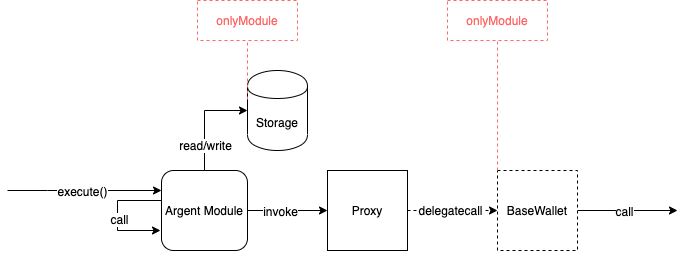
\includegraphics[width=\textwidth]{SC_Flow_3_x}
    \caption{Call flow in Argent}
\end{figure}

A second group of contracts implements the functionalities of the wallet:
\begin{itemize}
    \item \textbf{Proxy Wallet:} Lightweight proxy contract that delegates all calls to a Base Wallet library-like contract. There is one proxy deployed per wallet. Note that the rationale for using the Proxy-Implementation design pattern\footnote{ introduced by Nick Johnson in https://gist.github.com/Arachnid/4ca9da48d51e23e5cfe0f0e14dd6318f} is \emph{not} to enable wallet upgradability (we use upgradable modules/features for that) but simply to reduce the deployment cost of each new wallet.
    \item \textbf{Base Wallet:} The Base Wallet is a simple library-like contract implementing basic wallet functionalities used by proxy wallets (via delegatecalls), that are not expected to ever change. These functionalities include changing the owner of the wallet, (de)authorizating modules and performing (value-carrying) internal transactions to third-party contracts.
    \item \textbf{ArgentModule:} The different functionalities of the wallet are typically encapsulated in \emph{Modules}. Each module contract is used by all wallets to handle a specific set of operations (e.g. adding and revoking guardians). Modules are added in bundles by the Argent multisig and each bundle is given a unique version number. A wallet can then be upgraded by its owner to use a certain bundle of features (i.e. version number). The current version of the wallet has only one module the \emph{ArgentModule} which implements all the required functionalities.
    \item \textbf{Storages:} Modules store part of their states in a dedicated storage contract (see Section~\ref{sec:storage}).
\end{itemize}


%%%%%%%%%%%%%%%%%%%%%%%%%%%%%%%%%%%%%%%%%%%%%%%%%%%%%%%%%%%%%%%%%%%%%%%%%%%%%%%%%%%%%%%%%%%%%%%%%%%
\subsection{Upgradability}
\label{sec:upgradability}
Argent maintains an evolving set of registered \emph{Module} contracts. A subset of these \emph{Module} contracts are \emph{SimpleUpgrader} modules that define a migration path from a particular set of old modules to a new set of registered modules, i.e. it contains the list of modules to disable and the list of modules to enable to go from the old set to the new set. A user can perform an upgrade of their modules using one of the registered \emph{SimpleUpgrader} contracts.

%%%%%%%%%%%%%%%%%%%%%%%%%%%%%%%%%%%%%%%%%%%%%%%%%%%%%%%%%%%%%%%%%%%%%%%%%%%%%%%%%%%%%%%%%%%%%%%%%%%
\subsection{Storage}
\label{sec:storage}
To enable cost-efficient upgrades, the part of the wallet state that must be permanent across upgrades is stored on dedicated storage contracts. 

The current version of the wallet uses two storage contracts:
\begin{itemize}
    \item \textbf{Transfer Storage:} Used to store the trusted contacts of a wallet.
    \item \textbf{Guardian Storage:} Used to store the list of guardians of a wallet.
\end{itemize}

%%%%%%%%%%%%%%%%%%%%%%%%%%%%%%%%%%%%%%%%%%%%%%%%%%%%%%%%%%%%%%%%%%%%%%%%%%%%%%%%%%%%%%%%%%%%%%%%%%%
\subsection{Meta-Transactions}
\label{sec:meta-transactions}
Meta-Transactions are implemented in the abstract \emph{RelayerManager} from which the \emph{ArgentModule} inherit. It implements a permissionless method \emph{execute()} that is meant to be called by a relayer account. The relayer must pass to the \emph{execute()} function an intention and the signature(s) of this intention by the originator(s) of that intention. As described in Section~\ref{sec:eth-less-account}, this pattern allows ether-less accounts to perform operations on the wallet without the need to directly call the corresponding feature methods to do so.

%%%%%%%%%%%%%%%%%%%%%%%%%%%%%%%%%%%%%%%%%%%%%%%%%%%%%%%%%%%%%%%%%%%%%%%%%%%%%%%%%%%%%%%%%%%%%%%%%%%
\subsection{Modules}
As mentionned above, all the features of the Argent wallet are currently implemented in a single module. To structure the code, the \emph{ArgentModule} inherits from several abstract modules that each implements a coherent subset of the logic.

\subsubsection{RelayerManager}\label{RelayerManager}

The RelayerManager module is the entry point for meta-transactions. A relayer calls the \emph{execute()} method of the \emph{RelayerManager}, which validates the signatures provided, calls the required target method to run the business logic and optionally refunds the relayer's gas cost.

\subsubsection{SecurityManager}

The SecurityManager module contains all the logic related to the security of the wallet; namely adding and removing guardians, locking and unlocking the wallet, recovering and transfering ownership. 

\subsubsection{TransactionManager}

The TransactionManager module contains all the logic to execute multi-calls, including adding or removing a trusted contact, enabling or disabling a dapp registry, starting or closing a session, and executing multi-calls. 

\subsubsection{BaseModule}

The BaseModule is a base contract containing logic common to all modules.

\subsection{Dapp Registry}

TODO

\end{document}